%======================================================================
% ToolShield — Final Tables and Figures
% Generated from data/reports/latex_tables.txt (standard dataset)
% and data/reports/experiments_longschema/latex_tables.txt (long-schema)
%======================================================================

%----------------------------------------------------------------------
% Table 1: Main Results (Standard Dataset)
%----------------------------------------------------------------------
\begin{table}[htbp]
\centering
\caption{Model performance across split protocols on the standard dataset. Higher ROC-AUC and lower FPR@TPR are better.}
\label{tab:main-results}
\resizebox{\textwidth}{!}{%
\begin{tabular}{llcccc}
\toprule
Protocol & Model & ROC-AUC & PR-AUC & FPR@TPR90 & FPR@TPR95 \\
\midrule
S\_attack\_holdout & context\_transformer\_keep\_prompt & 0.999 & 0.999 & 0.000 & 0.010 \\
S\_attack\_holdout & context\_transformer\_naive & 0.998 & 0.999 & 0.000 & 0.010 \\
\midrule
S\_random & context\_transformer & 1.000 & 1.000 & 0.000 & 0.000 \\
S\_random & context\_transformer\_keep\_prompt & 1.000 & 1.000 & 0.000 & 0.000 \\
S\_random & context\_transformer\_naive & 1.000 & 1.000 & 0.000 & 0.000 \\
S\_random & heuristic & 0.714 & 0.872 & 1.000 & 1.000 \\
S\_random & heuristic\_score & 0.714 & 0.872 & 1.000 & 1.000 \\
S\_random & tfidf\_lr & 1.000 & 1.000 & 0.000 & 0.000 \\
S\_random & transformer & 0.998 & 0.998 & 0.000 & 0.040 \\
\bottomrule
\end{tabular}}
\end{table}

%----------------------------------------------------------------------
% Table 2: ASR Reduction (Standard Dataset)
%----------------------------------------------------------------------
\begin{table}[htbp]
\centering
\caption{ASR reduction at different TPR operating points on the standard dataset. Higher is better.}
\label{tab:asr-results}
\resizebox{\textwidth}{!}{%
\begin{tabular}{llcc}
\toprule
Protocol & Model & ASR Red.@TPR90 & ASR Red.@TPR95 \\
\midrule
S\_attack\_holdout & context\_transformer\_keep\_prompt & 93.6\% & 97.6\% \\
S\_attack\_holdout & context\_transformer\_naive & 91.2\% & 97.6\% \\
\midrule
S\_random & context\_transformer & 92.7\% & 100.0\% \\
S\_random & context\_transformer\_keep\_prompt & 92.7\% & 100.0\% \\
S\_random & context\_transformer\_naive & 94.4\% & 96.0\% \\
S\_random & heuristic & 100.0\% & 100.0\% \\
S\_random & heuristic\_score & 100.0\% & 100.0\% \\
S\_random & tfidf\_lr & 90.3\% & 96.8\% \\
S\_random & transformer & 94.4\% & 100.0\% \\
\bottomrule
\end{tabular}}
\end{table}

%----------------------------------------------------------------------
% Table 4: Inference Latency (Standard Dataset)
%----------------------------------------------------------------------
\begin{table}[htbp]
\centering
\caption{Warm inference latency per batch (100 samples), standard dataset, \texttt{S\_random} protocol. Lower is better.}
\label{tab:latency-results}
\begin{tabular}{lcc}
\toprule
Model & P50 (ms) & P95 (ms) \\
\midrule
context\_transformer\_keep\_prompt & 3997.70 & 4057.87 \\
context\_transformer\_naive & 2469.62 & 2512.38 \\
context\_transformer & 4126.69 & 4205.87 \\
heuristic & 1.39 & 1.52 \\
heuristic\_score & 1.53 & 1.63 \\
tfidf\_lr & 2.42 & 2.87 \\
transformer & 737.43 & 766.61 \\
\bottomrule
\end{tabular}
\end{table}

%----------------------------------------------------------------------
% Table 6: Long-Schema Stress Test (Production-Scale Approximation)
%----------------------------------------------------------------------
\begin{table}[htbp]
\centering
\caption{Long-schema truncation stress test (4\,000-char schemas, production-scale approximation). Prompt truncation and model performance under naive vs \texttt{keep\_prompt} strategies.}
\label{tab:longschema-stress}
\resizebox{\textwidth}{!}{%
\begin{tabular}{ll cc cccc cc}
\toprule
 & & \multicolumn{2}{c}{Truncation} & \multicolumn{4}{c}{Performance} & \multicolumn{2}{c}{Latency (ms)} \\
\cmidrule(lr){3-4} \cmidrule(lr){5-8} \cmidrule(lr){9-10}
Protocol & Strategy & Trunc.\% & Ret. Mean & ROC-AUC & PR-AUC & FPR@90 & FPR@95 & P50 & P95 \\
\midrule
S\_attack\_holdout & keep\_prompt & 0.0\% & 1.000 & 0.998 & 0.998 & 0.000 & 0.010 & 4527.48 & 4615.62 \\
S\_attack\_holdout & naive & 100.0\% & 0.000 & 0.455 & 0.541 & 0.920 & 0.950 & 4403.95 & 4859.30 \\
\midrule
S\_random & keep\_prompt & 0.0\% & 1.000 & 0.997 & 0.998 & 0.000 & 0.003$\pm$0.006 & 4579.35 & 4806.96 \\
S\_random & naive & 100.0\% & 0.000 & 0.479 & 0.657 & 0.900 & 0.960 & 4583.62 & 4872.23 \\
\bottomrule
\end{tabular}}
\end{table}

%----------------------------------------------------------------------
% Figure 1: Prompt Retention — Quartile Plot
%----------------------------------------------------------------------
\begin{figure}[htbp]
\centering
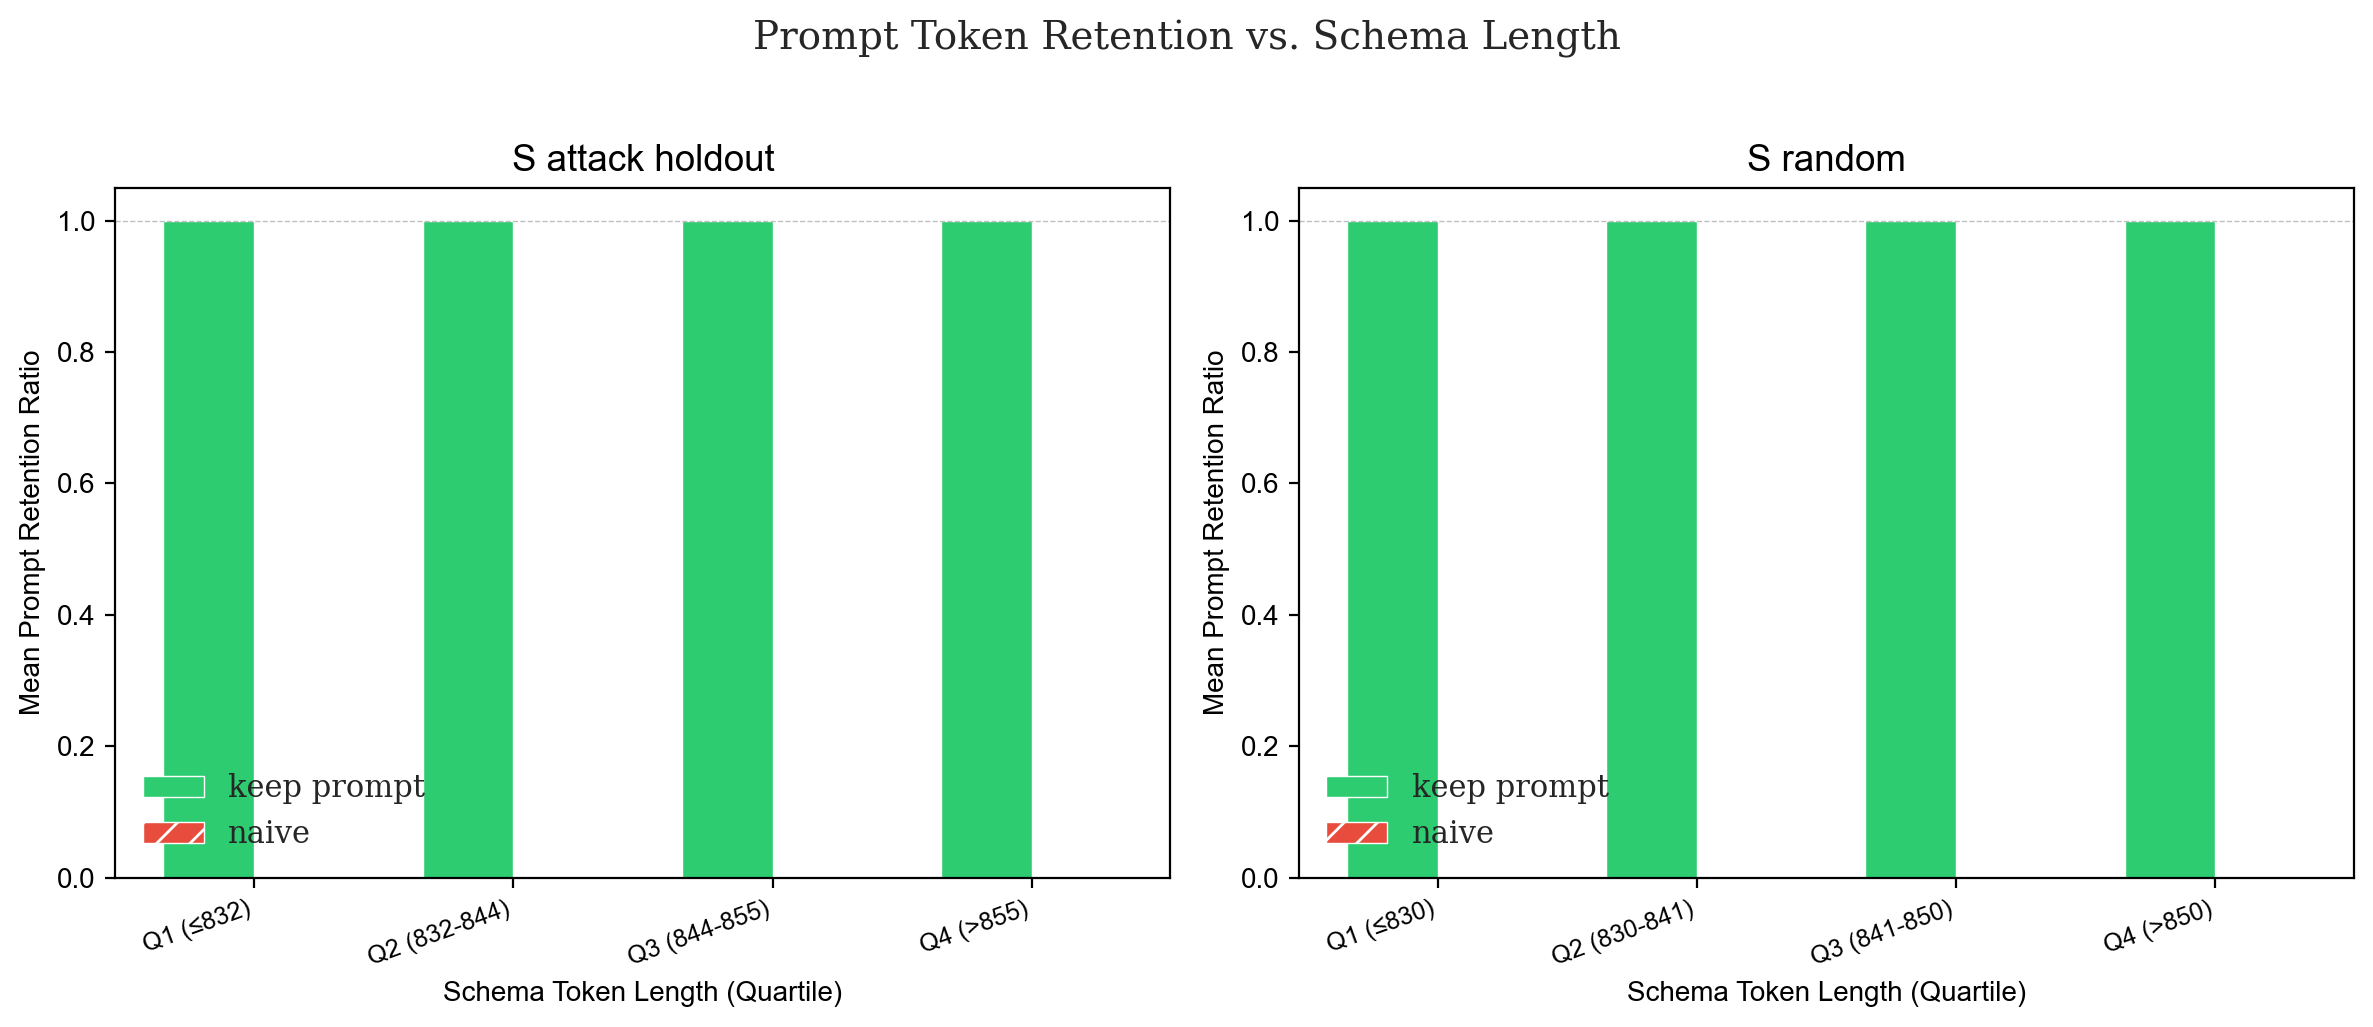
\includegraphics[width=\textwidth]{figures/prompt_retention_quartiles.png}
\caption{Prompt retention ratio by schema token length quartiles under production-scale schema lengths. Naive truncation collapses retention to zero across all bins, while \texttt{keep\_prompt} preserves the full prompt.}
\label{fig:prompt-retention-quartiles}
\end{figure}

%----------------------------------------------------------------------
% Figure 2: Prompt Retention — Decile Plot
%----------------------------------------------------------------------
\begin{figure}[htbp]
\centering
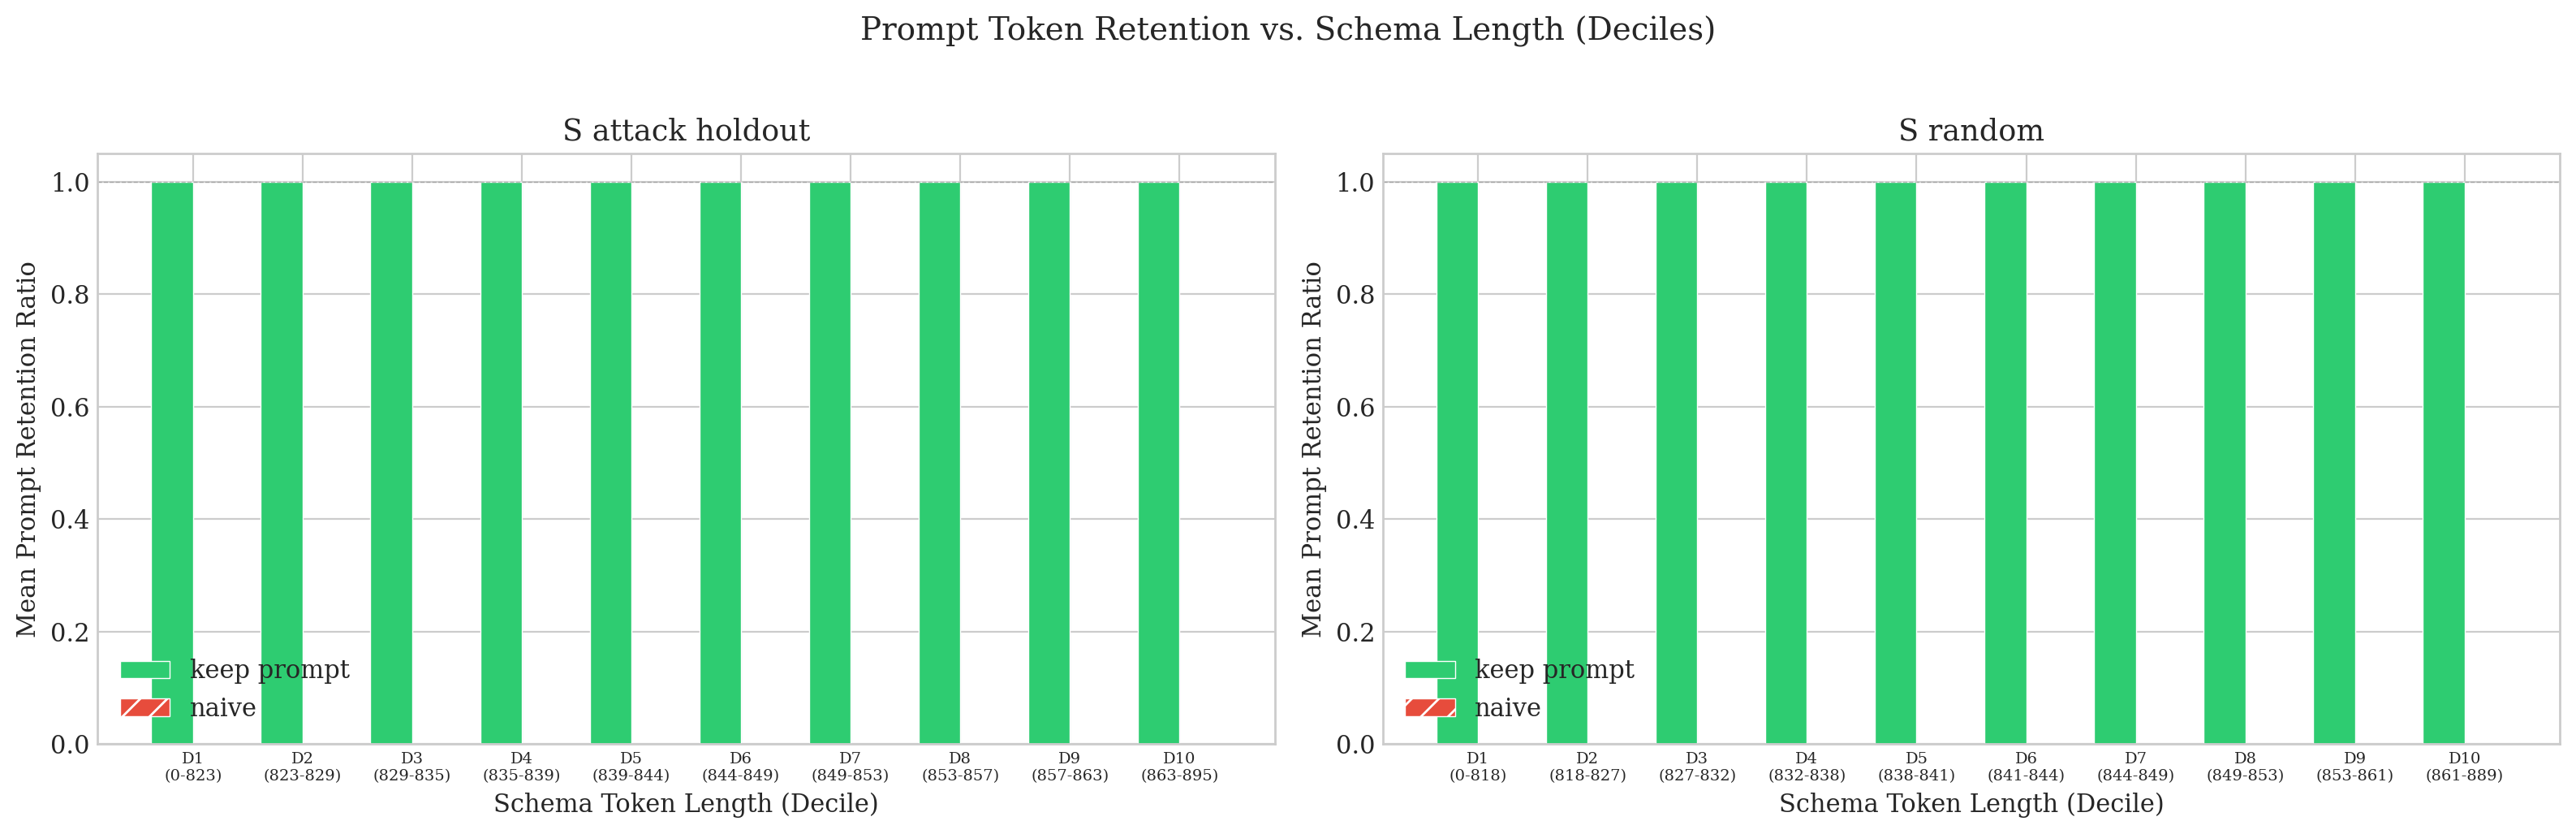
\includegraphics[width=\textwidth]{figures/prompt_retention_deciles.png}
\caption{Prompt retention ratio by schema token length deciles under production-scale schema lengths. Fine-grained view confirming that retention collapse under naive truncation is uniform across all schema length bins.}
\label{fig:prompt-retention-deciles}
\end{figure}
